\documentclass[main.tex]{subfiles}
\newcommand{\snzi}{\sum_{n=0}^{+\infty}}
\newcommand{\snii}{\sum_{n=0}^{+\infty}}

\begin{document}
\section{Principes}

\begin{figure}[h!]
\centering
\begin{subfigure}{.6\textwidth}
  \begin{tikzpicture}
    \sbEntree{A}
    \sbBlocL{E}{Échantilloneur}{A}
    \sbSortie{S}{E}
    \sbRelier{E}{S}
    \node[left=-1em] at (A) {
      \begin{tabular}{c}
        Signal\\ analogique \\
        à temps\\ continu
      \end{tabular}};
    \node[right=-1em] at (S) {
      \begin{tabular}{c}
        Signal\\ analogique \\
        à temps\\ continu
      \end{tabular}};
  \end{tikzpicture}
\end{subfigure}%
\begin{subfigure}{.4\textwidth}
  \begin{tikzpicture}
    \begin{axis}
      [axis lines = middle, width=8cm,
      xmin=0,xmax = 10,ymin=-2,ymax=3,
      ytick =\empty, ylabel={{\color{blue}$x_c(t)$}, {\color{red}$x_E(t)$}},
      xtick = {3,6,9},xticklabels={$T_e$,$2T_e$,$3T_e$},
      x tick label style={yshift={mod(\ticknum,2)*2em}}]
      \addplot+[smooth,no marks] plot coordinates{(0,2) (2,1.5) (3,2) (4,1) (5,-1.5)(6,-1.5)(7,0)(9,1)};
      \draw[dashed,red] (axis cs:3,0)-- (axis cs:3,2)node{$\bullet$}
      (axis cs:6,0)-- (axis cs:6,-1.5)node{$\bullet$}
      (axis cs:9,0) -- (axis cs:9,1)node{$\bullet$};
    \end{axis}
  \end{tikzpicture}
\end{subfigure}
\end{figure}

On prélève la valeur de $x_c(t)$ à un instant de l'ensemble discret $nT_e, n\in\N$.

\[x_E(t) = \snzi x_c(nT_e) \delta(t-nT_e) \]

\begin{rem}
$\snzi$ traduit la causalité, la distribution $\delta$ traduit la durée infiniment courte de l'échantillonnage (échantillonnage idéal)
\end{rem}
\pagebreak
Dans le domaine fréquentiel, on a donc
\begin{align*}
X_E(f) & = (X_c * TF [ \snzi \delta(t-nT_e) ])(f) \\
& = (X_c * TF [ \snii \delta(t-nT_e) ])(f) \quad \text{ avec } x_c(t) = 0 , t <0 \\
\text{Or, } TF [ \snzi \delta(t-nT_e) ] & = \snzi e^{-j2\pi f T_e} \\
&  = \frac{1}{T_e} \snzi \delta(f-\frac{n}{T_e})  \text{ d'après la formule de Poisson} \\
\text{ donc } X_E(f) & = F_e \snii X_c(f-nF_e)
\end{align*}

On répète donc le spectre de $x_c$ à tous les multiples de la fréquence d'échantillonnage.

\begin{figure}[H]
  \centering
  \begin{subfigure}{.5\textwidth}
\centering
    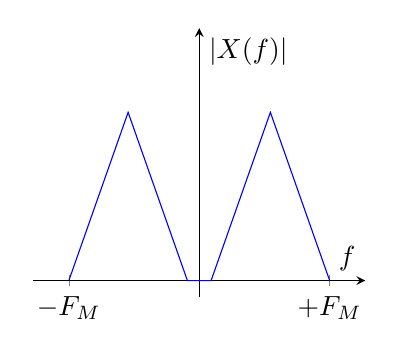
\begin{tikzpicture}
    \begin{axis}%
      [axis lines = middle,
      height = 5cm,
      xlabel = {$f$},
      ylabel = {$|X(f)|$},
      xmin = -7 ,xmax = 7, ymin = -0.1, ymax = 1.5,
      xtick = {-5.5,5.5},
      xticklabels = {$-F_M$, $+F_M$},
      ytick=\empty]
      \addplot+[no marks] plot coordinates {(-5.5,0) (-3,1) (-0.5,0) (0.5,0) (3,1) (5.5,0)};
    \end{axis}
  \end{tikzpicture}
  \caption{Spectre du signal continu}
\end{subfigure}%
  \begin{subfigure}{.5\textwidth}
    \centering
    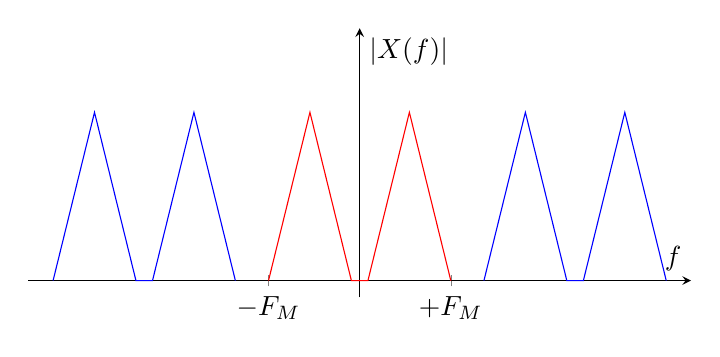
\begin{tikzpicture}
    \begin{axis}%
      [axis lines = middle,
      height = 5cm, width=10cm,
      xlabel = {$f$},
      ylabel = {$|X(f)|$},
      xmin = -20 ,xmax = 20, ymin = -0.1, ymax = 1.5,
      xtick = {-5.5,5.5},
      xticklabels = {$-F_M$, $+F_M$},
      ytick=\empty]
      \addplot+[no marks, red] plot coordinates {
         (-5.5,0) (-3,1) (-0.5,0) (0.5,0) (3,1) (5.5,0)
      };
      \addplot+[no marks,blue] plot coordinates {
        (-18.5,0) (-16,1) (-13.5,0) (-12.5,0) (-10,1) (-7.5,0)
       };
\addplot+[no marks,blue] plot coordinates {
        (7.5,0) (10,1) (12.5,0) (13.5,0) (16,1) (18.5,0)
      };
    \end{axis}
  \end{tikzpicture}
  \caption{Spectre du signal échantilloné}
\end{subfigure}\\
  \begin{subfigure}{.5\textwidth}
\centering
  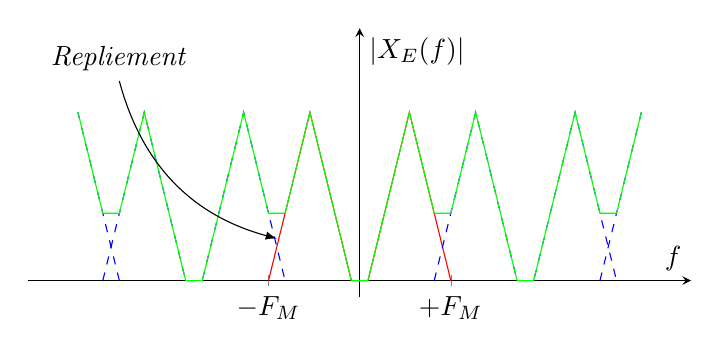
\begin{tikzpicture}
    \begin{axis}%
      [axis lines = middle,
      height = 5cm, width=10cm,
      xlabel = {$f$},
      ylabel = {$|X_E(f)|$},
      xmin = -20 ,xmax = 20, ymin = -0.1, ymax = 1.5,
      xtick = {-5.5,5.5},
      xticklabels = {$-F_M$, $+F_M$},
      ytick=\empty]
      \addplot+[no marks, red] plot coordinates {
         (-5.5,0) (-3,1) (-0.5,0) (0.5,0) (3,1) (5.5,0)
      };
      \addplot[no marks, dashed ,blue] plot coordinates {
        (-15.5,0) (-13,1) (-10.5,0) (-9.5,0) (-7,1) (-4.5,0)};
      \addplot[no marks, dashed ,blue] plot coordinates {
        (4.5,0) (7,1) (9.5,0) (10.5,0) (13,1) (15.5,0)
      };
      \addplot[no marks, dashed ,blue] plot coordinates {
        (14.5,0) (17,1)};
      \addplot[no marks, dashed ,blue] plot coordinates {
        (-14.5,0) (-17,1)};

      \addplot[no marks,green] plot coordinates {
        (-17,1) (-15.5,0.4) (-14.5,0.4)
        (-13,1) (-10.5,0) (-9.5,0) (-7,1)
        (-5.5,0.4) (-4.5,0.4) (-3,1) (-0.5,0) (0.5,0) (3,1)
        (4.5,0.4)(5.5,0.4) (7,1) (9.5,0) (10.5,0) (13,1)
        (14.5,0.4) (15.5,0.4) (17,1)};

  \coordinate (R) at (axis cs: -5,0.25);
    \end{axis}
    \draw[latex-] (R)  to[bend left] ++(-2,2) node[above]{\textit{Repliement}};

  \end{tikzpicture}
  \caption{Repliement de spectre}
\end{subfigure}
\end{figure}

\begin{thm}[Théorème de Shannon]
La fréquence d'échantillonnage doit être au moins 2 fois supérieure à la fréquence maximale du spectre du signal échantillonné.
\[ F_e > 2 F_M \]
\end{thm}

Comme le signal $x_c(t)$ est a priori aléatoire, on ne peut pas forcément garantir de connaître la valeur de sa fréquence maximale $F_M$. On ajoute donc un filtre anti-repliement (\emph{anti-aliasing}) avant l'échantillonnage pour garantir le critère de Shannon.

\begin{figure}[H]
  \centering
  \begin{circuitikz}
    \draw (0,0) node[left]{$x_c(t)$} to[lowpass] ++ (2,0)  to[spst,l=$T_e$] ++(2,0) node[inputarrow]{} node[right]{$x_E(t)$};
  \end{circuitikz}
  \caption{Utilisation d'un filtre antirepliement }
\end{figure}

\begin{rem}
Le filtre anti-repliement est un filtre passe-bas de fréquence de coupure (bande passante) $\frac{F_e}{2}$
\end{rem}

\section{Reconstitution d'un signal}
Pour retrouver le signal analogique à temps continu, si le théorème de Shannon est respecté, il suffit de faire un filtrage passe-bas sur une bande de fréquence $F_M$ de $x_E(t)$ :

\begin{figure}[H]
  \centering
    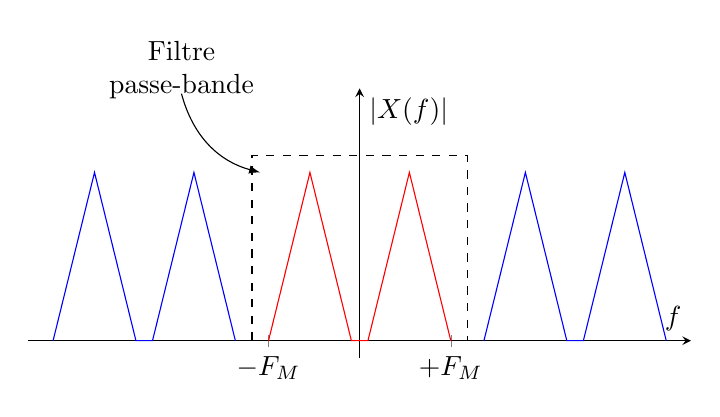
\begin{tikzpicture}
    \begin{axis}%
      [axis lines = middle,
      height = 5cm, width=10cm,
      xlabel = {$f$},
      ylabel = {$|X(f)|$},
      xmin = -20 ,xmax = 20, ymin = -0.1, ymax = 1.5,
      xtick = {-5.5,5.5},
      xticklabels = {$-F_M$, $+F_M$},
      ytick=\empty]
      \addplot+[no marks, red] plot coordinates {
         (-5.5,0) (-3,1) (-0.5,0) (0.5,0) (3,1) (5.5,0)
      };
      \addplot+[no marks,blue] plot coordinates {
        (-18.5,0) (-16,1) (-13.5,0) (-12.5,0) (-10,1) (-7.5,0)
       };
\addplot+[no marks,blue] plot coordinates {
        (7.5,0) (10,1) (12.5,0) (13.5,0) (16,1) (18.5,0)
      };
      \addplot[no marks, dashed, black] plot coordinates {
        (-6.5,0) (-6.5,1.1) (6.5,1.1) (6.5,0)
      };
      \coordinate (A) at (axis cs:-6,1);
    \end{axis}
    \draw[latex-] (A) to[bend left] ++(-1,1) node[above=-0.7em]{
      \begin{tabular}{c}
Filtre\\ passe-bande
      \end{tabular}
};
  \end{tikzpicture}
  \caption{Reconstitution du signal continu}
\end{figure}

Formellement, on peut considérer la transformée de Laplace :
\[ TL[x_E(t)] = X_E(p) = X_c(p) * TL[\snii \delta(t-nT_e)] \]

Or, \[TL[\snii \delta(t-nT_e)] = \snii  e^{-npT_e} = \snii z^{-n} \]

donc finalement
\[X_c(z) = \snii x_c(nT_e)z^{-n}\]


\section{Échantillonneur bloqueur}

Dans la réalité, la valeur échantillonnée est conservée sur un temps de blocage $\tau \leq T_e$. En pratique, $\tau = T_e$.\\


\begin{figure}[H]
  \centering
    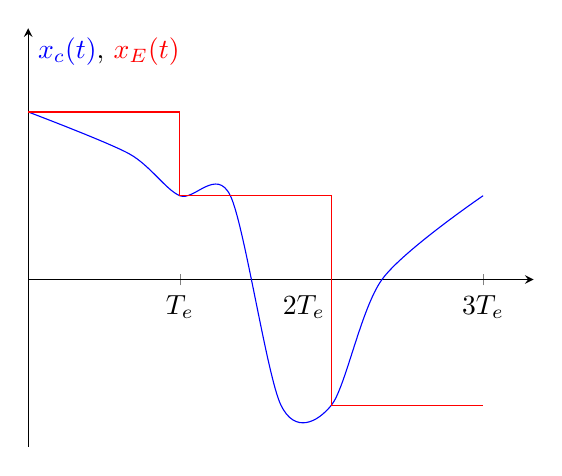
\begin{tikzpicture}
    \begin{axis}
      [axis lines = middle, width=8cm,
      xmin=0,xmax = 10,ymin=-2,ymax=3,
      ytick =\empty, ylabel={{\color{blue}$x_c(t)$}, {\color{red}$x_E(t)$}},
      xtick = {3,6,9},xticklabels={$T_e$,$2T_e$,$3T_e$},
      x tick label style={xshift={-mod(\ticknum,2)*1em}}]
      \addplot+[smooth,no marks] plot coordinates{(0,2) (2,1.5) (3,1) (4,1) (5,-1.5)(6,-1.5)(7,0)(9,1)};

      \addplot+[no marks, red] plot coordinates
      {(0,2) (3,2) (3,1) (6,1)  (6,-1.5) (9,-1.5)};
    \end{axis}
  \end{tikzpicture}
  \caption{Echantillonneur bloqueur}
\end{figure}


On écrit donc \[ x_E(t) = \snzi x_c(nT_e)P_{\tau}(t-nT_e), \quad P_{\tau} \text{ fonction porte } P_{\tau} (t) =
  \begin{cases}
    1 & \text{ si } 0 \leq t \leq \tau\\
    0 & \text{ sinon}
\end{cases}
\]

On peut également écrire
\[x_E(t) = (\snii x_c(nT_e)\delta(t-nt_e)) * P_{\tau}(t) \]

d'où
\[X_E(f) = (F_E \snii X_c(f-nF_e)) TF [P_{\tau}(t)]\]

Comme $TF [P_{\tau}(t)] = \tau e^{-j2\pi f \tau} \sinc(\pi f \tau)$,

\[X_E(f) = \tau F_E \snii X_c(f-nF_e) e^{-j2\pi f \tau} \sinc(\pi f \tau) \]

%\img{0.5}{1/10.png}

Autour de $f=0$, le spectre est peu modifié. Autour des autres multiples de $F_e$, le spectre sera atténué par le sinus cardinal.

\begin{rem}
Si $\tau = T_e$, on a une atténuation par le sinus cardinal en $f=\frac{F_e}{2}$ (limite de Shannon) de 3.9dB (non négligeable)
\end{rem}

\section{Techniques de mise en oeuvre}

\subsection{L'échantillonneur}

Il faut un interrupteur électronique commandable. Typiquement, cette fonction est réalisée par un transistor à effet de champ de type MOSFET (\emph{Metal Oxyde Semi-conductor Field Effect Transistor})


MOSFET à canal N (charges négatives qui constituent le canal) de type \emph{Normally Off} (le canal n'existe pas si on n'applique pas le bon type de tension) de symbole suivant :

\begin{center}
  \begin{circuitikz}
    \draw (0,0) node[nmos,rotate=-90](N){}
    (N.G)node[anchor=south]{G :  grille}
    (N.S)node[anchor=north east]{S :source}
    (N.D)node[anchor=north west]{D : drain};
  \end{circuitikz}
\end{center}

\paragraph{Principe de fonctionnement :}

former (ou faire disparaître) un canal de transmission en électrons entre les électrodes de drain et de source grâce au champ électrique induit dans l'oxyde par la tension grille-souce $V_{GS}$.

La conductivité (donc résistivité) du canal est contrôlée par $V_{GS}$. L'accélération des électrons est contrôlée par $V_{DS}$ : $V_{DS}$ contrôle le courant de drain $I_D$ par déplacement d'électrons de la source au drain, d'où $I_D(V_{DS},V_{GS})$.\\

\paragraph{Caractéristiques électriques}

\begin{figure}[H]
  \centering
  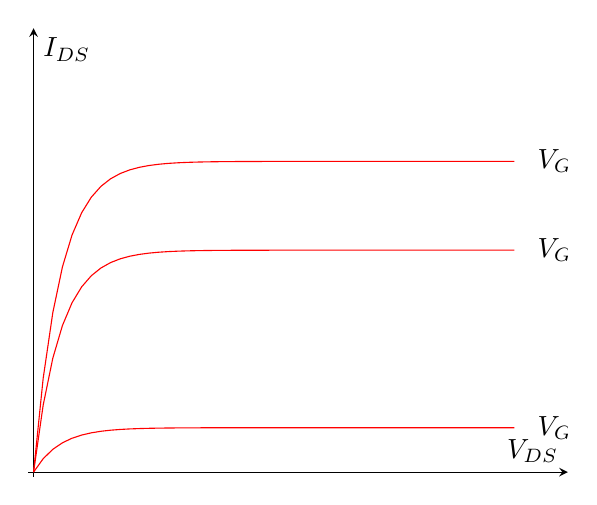
\begin{tikzpicture}
    \begin{axis}
      [axis lines = middle,
      xmin=-0.1,xmax =10,ymin=-0.1,ymax=10,
      domain=0:9,ticks=none,samples=51,
      xlabel=$V_{DS}$,ylabel=$I_{DS}$]
      \addplot[no marks,red,]{1*(1-exp(-x/0.5))};
      \addplot[no marks,red,]{5*(1-exp(-x/0.5))};
      \addplot[no marks,red,]{7*(1-exp(-x/0.5))};
      \node  at (axis cs:10,1) {$V_{GS1}$};
      \node  at (axis cs:10,5) {$V_{GS5}$};
      \node  at (axis cs:10,7) {$V_{GS3}$};
    \end{axis}
  \end{tikzpicture}
  \caption{Caractéristique d'un transistor NMOS}
\end{figure}
\begin{itemize}
\item Si $V_{GS}=0$ transistor bloqué tant que $0<V_{GS}<V_T$, $V_T$ tension de seuil (pour l'apparition d'un canal en électrons entre source et drain, $V_T$  pour \emph{threshold}). On est à l'état État off.
  On est alors en régime ohmique (si $V_{GS}$ augmente, la densité des électrons augmente donc la résistance du canal diminue).\\
\item si $V_{DS}\gg V_{GS}-V_T$ est assez grand on se place dans la \emph{zone de saturation}  et on a une source de courant idéale.
\[
  I_{D} = \frac{\beta}{2}\left( V_{GS}-V_T\right)^2
\]

\item si $V_{DS}< V_{GS}-V_{T}$ on est dans la \emph{zone ohmique}.
\[
  I_{D} = \beta \left( V_{GS}-V_T-\frac{1}{2}V_{DS}\right)V_{DS}
  \overset{V_{DS}\ll V_{GS}-V_{T} }{\simeq}
   \beta (V_{GS}-V_T)V_{DS}
\]

\end{itemize}

%\includegraphics[width=0.5\textwidth]{1/12.png}

\paragraph{Structure physique}

\begin{figure}[H]
  \centering

  \caption{Structure interne d'un transistor mos}
\end{figure}


Les 2 zones de Si dopées N sont des réservoirs à électrons, séparées par la longueur de la grille $L_G$, par une zone de Si dopée P où les porteurs de courant sont des trous (charges positives).

À l'interface P/N il y a une barrière d'énergie potentielle qui empêche les électrons de passer dans la zone P et les trous dans la zone N.

Si on applique $V_{GS}>0$, on crée un champ électrique dans l'oxyde dans le sens de la grille vers S, qui repousse les trous vers le fond de la plaquette et attire les électrons des réservoirs de source et de drain.

Si $V_{GS}>V_T$ tous les trous ont disparu de la zone sous l'oxyde et on y a créé un canal riche en électrons de S à D.


Mais $R_{on} = \frac{K}{V_{GS}-V_T}$ pour $V_{GS} \geq V_T$ la résistance du canal pour $V_{DS} \approx 0$.

On vise l'état On : $V_G = V_{DD}$ mais $V_{GS}=V_{DD}-x_c$.

MOSFET passant équivaut à $V_{GS} \geq V_T$ soit $x_c \leq V_{DD}-V_T$.

\begin{figure}[H]
  \centering
  \begin{tikzpicture}
    \begin{axis}
      [axis lines = middle,
      xmin=-0.1,xmax =10,ymin=-0.1,ymax=10,
      domain=0:2.99,samples=51, height=5cm,
      xlabel=$x_c$,ylabel=$R_{OM}$,
      ytick=\empty,
      xtick = {3}, xticklabels={$V_{DD}-V_{T}$}]
      \addplot[no marks,red,]{-2/(x-3)};
      \addplot[no marks, dashed, black] plot coordinates{(3,0) (3,9.9)};

    \end{axis}
  \end{tikzpicture}
  \caption{Caractéristique d'un transistor NMOS}
\end{figure}

\textbf{Comment améliorer la gamme de variation possible de $x_c$ ?} \\

Le MOSFET à canal P a une zone sous sa grille dopé N et 2 réservoirs dopés P. On le choisit conducteur pour $V_{GS} < -V_T < 0$. On a alors un interrupteur CMOS (C pour complementary)
\begin{figure}[H]
  \centering
  \begin{circuitikz}
    \draw (0,1) node[nmos,rotate=-90](N){} (0,-1) node[pmos,rotate=90](P){}
    (N.S) -- (P.S) node[midway](A){} (P.D)--(N.D)node[midway](B){}
    (A) to[short,-o] ++(-1,0)node[left]{$x_c$} (B) to[short,-o] ++(1,0) node[right]{$x_e(t)$}
    ;\end{circuitikz}
  \caption{Interrupteur CMOS}
\end{figure}
À l'état passant de l'interrupteur CMOS :
\begin{itemize}
\item $R_{ON_N} = \frac{K}{V_{GS_N}-V_T} = \frac{K}{V_{DD}-x_C-V_T}$ pour $x_c \leq V_{DD}-V_T$
\item $R_{ON_P} = \frac{K}{V_{GS_P}+V_T} = \frac{K}{-x_c+V_T}$ pour $x_c > V_T$
\end{itemize}

Avec $R_{ON_N} // R_{ON_P}$ la résistance globale est quasiment constante quand l'interrupteur CMOS est passant.
\begin{figure}[H]
  \centering
  \begin{tikzpicture}
    \begin{axis}
      [axis lines = middle,
      xmin=-0.1,xmax =10,ymin=-0.1,ymax=10,
      samples=51, height=5cm, domain = 1.01:6.99,
      xlabel=$x_c$,ylabel=$R_{OM}$,
      ytick=\empty,
      xtick = {9}, xticklabels={$V_{DD}-V_{T}$}]
      \addplot[no marks,black,dashed]{-1/(x-7)+1};
      \addplot[no marks,blue,dashed]{1/(x-1)+1};
      \addplot[no marks,red,smooth] plot coordinates {(1,1) (4,1.3) (7,1)};

    \end{axis}
  \end{tikzpicture}
  \caption{Résistance d'un interrupteur CMOS}
\end{figure}

\subsection{Le bloqueur}
\begin{figure}[H]
  \centering
  \begin{circuitikz}
    \draw (0,0) node[op amp](oa){}
    (oa.-) -- ++(0,1) -| (oa.out) to[short,-o] ++(1,0)node[right]{$x_e(t)$}
    (oa.+) -- ++(-1,0) coordinate(A) to[C] ++(0,-2) node[ground]{}
    (A) ++ (-2,0)node[left]{$x_c(t)$} to[spst,o-] (A)
  ;\end{circuitikz}
  \caption{Schéma électrique d'un échantilloneur bloqueur}
\end{figure}

L’échantillonneur est un interrupteur électronique contrôlé par une horloge de période $T_e = \frac{1}{F_e}$\\
La capacité est utilisée pour le "blocage".\\
Le suiveur est optionnel et permet d'avoir une tension $x_e(t)$ non perturbée par ce qui suit.\\

Que peut-on utiliser comme interrupteur?\\

\begin{figure}[H]
  \centering
  \begin{circuitikz}
    \draw (0,1) node[nmos,rotate=-90](N){} (0,-1) node[pmos,rotate=90](P){}
    (N.S) -- (P.S) node[midway](A){} (P.D)--(N.D)node[midway](B){}
    (A) to[short,-o] ++(-1,0)node[left]{$x_c$} (B) to[short,-o] ++(1,0) node[right]{$x_e(t)$}
    (N.G) node[above]{$horloge$}
    (P.G) node[below]{$\overline{horloge}$}
    ;\end{circuitikz}
  \caption{Interrupteur CMOS}
\end{figure}


Les MOSFET sont passants quand l'horloge est à l'état logique haut, c'est à dire que la tension $V_{DD}$ est positive par rapport à la masse.

À l'état passant, un MOSFET est équivalent à une résistance $R_{on}$.\\

$V_t$ est la tension seuil du MOSFET à canal N au niveau de $V_{GS}$ pour le mettre à l'état passant. On utilise donc deux MOSFET pour limiter la résistance $R_{on}$.\\

Les interrupteur CMOS sont intégrables sur silicium en même temps que la capacité MOS réalisant la fonction de blocage, de même que le suiveur.
\[x_E(t) = \left(\sum_{n=0}^{\infty} x_c(nT_e)\delta(t-nT_e)\right)*P_{\tau}(t)\]

En effectuant la transformée de Fourier de ce signal on a:
\[X_E(f) = TF(x_E(t)) = (F_e \sum_{n=-\infty}^{\infty} X_C(f-nF_e)).\tau exp(-j\pi f \tau)sinc(\pi f \tau)\]
On fait attention à ce que $F_e$ vérifie la condition de Shannon. $F_e$ doit être supérieure au double de la fréquence maximale du spectre de $x_C(t)$.\\
\begin{figure}[H]
  \centering
  \begin{subfigure}{0.5\textwidth}
    \centering
    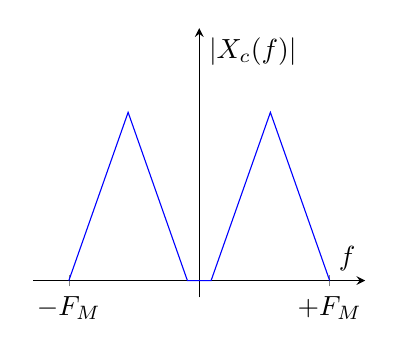
\begin{tikzpicture}
    \begin{axis}%
      [axis lines = middle,
      height = 5cm,
      xlabel = {$f$},
      ylabel = {$|X_c(f)|$},
      xmin = -7 ,xmax = 7, ymin = -0.1, ymax = 1.5,
      xtick = {-5.5,5.5},
      xticklabels = {$-F_M$, $+F_M$},
      ytick=\empty]
      \addplot+[no marks] plot coordinates {(-5.5,0) (-3,1) (-0.5,0) (0.5,0) (3,1) (5.5,0)};
    \end{axis}
    \end{tikzpicture}
  \end{subfigure}\\
  \begin{subfigure}{\textwidth}
    \centering
    \begin{tikzpicture}
    \begin{axis}
    [axis lines = middle,
      height = 5cm,width=15cm,
      xlabel = {$f$},
      ylabel = {$|X_e(f)|$},samples=200,
      xmin = -20 ,xmax = 20, ymin = -0.1, ymax = 3.5,
      xtick = {-5.5,5.5},
      xticklabels = {$-F_M$, $+F_M$},
      domain = -20:20,
      ytick=\empty]
      \addplot+[no marks] plot coordinates
      {(-5.5,0) (-3,1) (-0.5,0) (0.5,0) (3,1) (5.5,0)};
      \addplot+[no marks,blue] plot coordinates
      {(-18.5,0) (-16,0.2) (-13.5,0) (-12.5,0)(-12,0.2) (-10.5,0)(-8,0.5) (-7.5,0)};
      \addplot+[no marks,blue] plot coordinates
      {(7.5,0) (8,0.5)(10.5,0)(12,0.2) (12.5,0) (13.5,0) (16,0.2) (18.5,0)
      };

      \addplot+[no marks, dotted,black]{abs(3*sin(deg(x)*0.3)/(x*0.3)};
    \end{axis}
  \end{tikzpicture}

  \end{subfigure}
  \caption{Allure spectrale des signaux}
\end{figure}

\end{document}

%%% Local Variables:
%%% mode: latex
%%% TeX-master: "main"
%%% End:
